% Provenance (never printed): cycle 3 / 6e "La planete Terre" (water in the
% ground, groundwater, springs and wells; resource); see
% sources/book1/PROVENANCE.md. Book 1, grade 6, chapter 5.
% Vocabulary guard: "sediment" not before g7.4; the water cycle is recalled
% from the physics book (prose only).
\chapter{ज़मीन के नीचे का पानी}\label{ch:g6:water-underground}

गर्मी के एक गरम दिन खेत सूखे पड़े हैं और नालों में पानी कम है। फिर भी एक \omterm{def:g1:landscapes-around-us:landform}{पहाड़ी}
की तलहटी में ज़मीन से पानी लगातार ऊपर निकलता रहता है, ठंडा और साफ़, जैसे सारी
सर्दियों में निकलता रहा था, और एक कुंड भर देता है। हफ़्तों से \omterm{def:g4:clouds-rain-snow:precipitation}{बारिश} नहीं हुई है।
यह पानी कहाँ से आता है, और \omterm{def:g3:stones-pebbles-sand:rock}{चट्टान} से बाहर कैसे निकलता है?

\begin{omfigure}
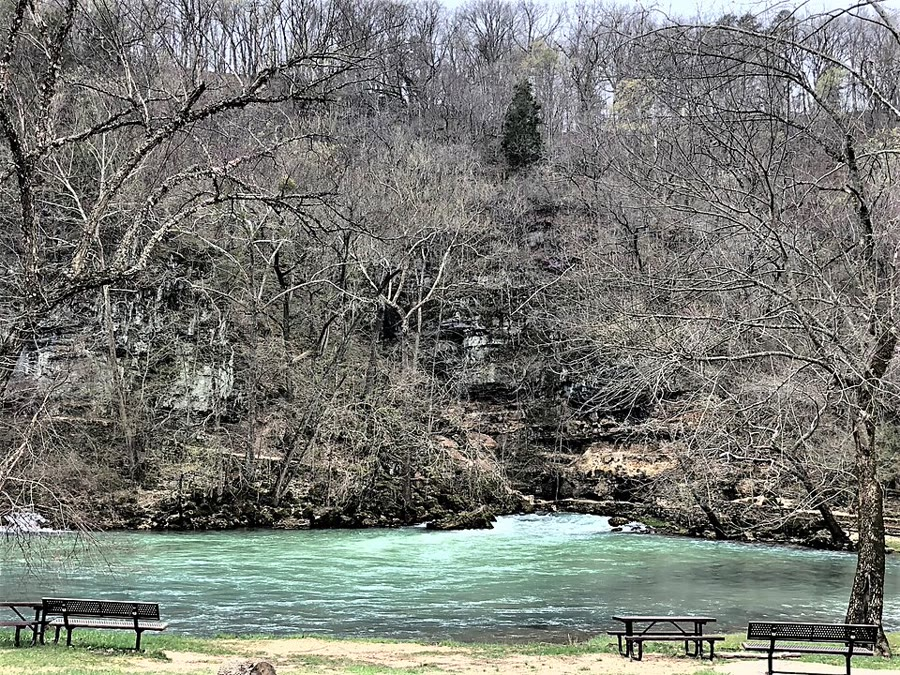
\includegraphics[width=0.72\linewidth]{images/book1/g6-big-spring.jpg}

{\small एक चट्टानी कगार की तलहटी में एक \omterm{def:g6:water-underground:spring}{सोता} फूटता है और एक कुंड भर देता है: बिग
स्प्रिंग, मिसूरी (संयुक्त राज्य अमेरिका)। (फ़ोटो: जॉनस्टन9494, CC BY-SA 4.0,
विकिमीडिया कॉमन्स के ज़रिए।)}
% ledger: commons:big-spring
\end{omfigure}

\begin{recall}
पृथ्वी का लगभग सारा पानी \omterm{def:g2:water-on-earth:salt-fresh}{खारा पानी} है; \omterm{def:g2:water-on-earth:salt-fresh}{मीठा पानी} उसका एक छोटा हिस्सा है, जो
ज़्यादातर बर्फ़ के रूप में और ज़मीन के नीचे रखा है
(\cref{ch:g2:water-on-earth})। बलुआ पत्थर और चूना पत्थर जैसी \omterm{def:g3:stones-pebbles-sand:rock}{चट्टानें} आपस में
चिपके कणों या सीपियों से बनी होती हैं, जबकि चिकनी मिट्टी और शेल बहुत महीन
कणों से बने होते हैं (\cref{ch:g6:rocks-and-minerals})। भौतिकी की किताब में
तुमने जल चक्र में पानी का पीछा किया है: वह \omterm{def:g2:water-on-earth:ocean}{समुद्रों} से वाष्पित होता है, \omterm{def:g4:clouds-rain-snow:cloud}{बादलों}
में संघनित होता है और \omterm{def:g4:clouds-rain-snow:precipitation}{बारिश} या बर्फ़ बनकर वापस गिरता है।
\end{recall}

\section{बारिश ज़मीन में रिसती है}

जब ज़मीन पर \omterm{def:g4:clouds-rain-snow:precipitation}{बारिश} गिरती है, तो पानी तीन रास्ते ले सकता है। उसका एक हिस्सा
वाष्पित होकर वापस हवा में चला जाता है। एक हिस्सा सतह के ऊपर से, ढलानों से नीचे,
नालों और \omterm{def:g1:landscapes-around-us:water}{नदियों} में बह जाता है: यह \emph{अपवाह} है। बाकी पानी ज़मीन में
रिस जाता है।

\begin{definition}[अंतःस्यंदन]\label{def:g6:water-underground:infiltration}
\emph{अंतःस्यंदन}\index{अंतःस्यंदन} \omterm{def:g4:clouds-rain-snow:precipitation}{बारिश} के पानी, या पिघली बर्फ़ के पानी, का
मिट्टी से होते हुए ज़मीन में और नीचे \omterm{def:g3:stones-pebbles-sand:rock}{चट्टानों} तक रिसना है।
\end{definition}

कितना पानी रिसता है, यह ज़मीन पर निर्भर करता है। खड़ी ढलान पर, नंगी या सख़्त
ज़मीन पर, सड़क या कार पार्किंग पर, या जब मिट्टी पहले से भीगी हो, तो ज़्यादातर
पानी बह जाता है। हल्की ढलान पर, घास और पेड़ों के नीचे, रेतीली मिट्टी पर, उसके
ज़्यादा हिस्से को रिसने का समय मिलता है।

\begin{omfigure}
\begin{tikzpicture}[x=1cm, y=1cm]
  % rain
  \foreach \x in {0.3,0.9,...,10.5} \draw[blue!55, thick] (\x,3.9) -- (\x-0.15,3.45);
  % ground: field on the left (gentle), road and town on the right
  \fill[brown!30] (0,0) -- (0,2.2) -- (5.2,1.9) -- (5.6,1.85) -- (10.8,1.1) -- (10.8,0) -- cycle;
  \draw[green!50!black, line width=2.5pt] (0,2.2) -- (5.2,1.9);
  \fill[gray!70] (5.6,1.85) -- (10.8,1.1) -- (10.8,0.98) -- (5.6,1.73) -- cycle;
  \foreach \x in {0.4,1.0,...,4.6} \draw[green!45!black, thick] (\x,{2.2-0.058*\x}) -- ++(0.05,0.28) (\x,{2.2-0.058*\x}) -- ++(-0.06,0.24);
  % infiltration arrows in the field
  \foreach \x in {0.8,1.9,3.0,4.1} \draw[->, blue!70!black, very thick] (\x,{2.0-0.058*\x}) -- ++(0,-1.0);
  \node[font=\scriptsize, blue!70!black, align=center, fill=brown!30] at (2.45,0.45) {अंतःस्यंदन: पानी ज़मीन में रिसता है};
  % run-off on the road
  \draw[->, blue!70!black, very thick] (6.0,2.05) -- (10.3,1.45);
  \node[font=\scriptsize, blue!70!black, align=center] at (8.3,2.3) {अपवाह: पानी बह जाता है};
  \node[font=\scriptsize, align=center] at (8.3,0.5) {सड़क: सख़्त ज़मीन,\\ थोड़ा ही पानी रिसता है};
  \node[font=\scriptsize] at (2.45,2.75) {घास का मैदान};
  % evaporation
  \draw[->, gray, thick, decorate, decoration={snake, amplitude=1.2pt, segment length=5pt}] (4.9,2.2) -- (4.9,3.3);
  \node[font=\scriptsize, gray!60!black, anchor=west] at (5.0,3.0) {वाष्पन};
\end{tikzpicture}

{\small \omterm{def:g4:clouds-rain-snow:precipitation}{बारिश} के पानी के तीन रास्ते। घास के मैदान में उसका बड़ा हिस्सा रिस जाता
है; सड़क पर ज़्यादातर पानी बह जाता है।}
\end{omfigure}

\section{सरंध्र और पारगम्य चट्टानें}

सूखी \omterm{def:g3:stones-pebbles-sand:sand}{रेत} की एक मुट्ठी को आवर्धक लेंस से देखो: कणों के बीच नन्ही-नन्ही खाली
जगहें हैं। उस पर पानी डालो तो पानी इन जगहों को भर देता है। बहुत-सी \omterm{def:g3:stones-pebbles-sand:rock}{चट्टानें}
ऐसी ही हैं: उनमें कणों के बीच छोटे-छोटे छेद भरे होते हैं, या पतली दरारें
होती हैं।

\begin{definition}[सरंध्रता]\label{def:g6:water-underground:porosity}
किसी \omterm{def:g3:stones-pebbles-sand:rock}{चट्टान} के \emph{रंध्र}\index{रंध्र} उसके कणों के बीच और उसकी दरारों में
खाली जगहें हैं। रंध्रों वाली \omterm{def:g3:stones-pebbles-sand:rock}{चट्टान} \emph{सरंध्र}\index{सरंध्र} होती है। उसकी
\emph{सरंध्रता}\index{सरंध्रता} उसके आयतन का वह हिस्सा है जो रंध्रों से बना है,
और उसे प्रतिशत में लिखा जाता है।
\end{definition}

\begin{definition}[पारगम्यता]\label{def:g6:water-underground:permeability}
कोई \omterm{def:g3:stones-pebbles-sand:rock}{चट्टान} \emph{पारगम्य}\index{पारगम्य} होती है जब पानी उसमें से होकर बह
सकता है, क्योंकि उसके \omterm{def:g6:water-underground:porosity}{रंध्र} काफ़ी बड़े हैं और एक-दूसरे से जुड़े हैं। वह
\emph{अपारगम्य}\index{अपारगम्य} होती है जब पानी उसमें से होकर नहीं बह सकता।
\emph{पारगम्यता}\index{पारगम्यता} यह है कि पानी किसी \omterm{def:g3:stones-pebbles-sand:rock}{चट्टान} में से कितनी
आसानी से बहता है।
\end{definition}

ये दोनों बातें एक नहीं हैं। चिकनी मिट्टी बहुत \omterm{def:g6:water-underground:porosity}{सरंध्र} है: उसका आधा आयतन
\omterm{def:g6:water-underground:porosity}{रंध्रों} से बना है। पर उसके \omterm{def:g6:water-underground:porosity}{रंध्र} इतने नन्हे हैं कि पानी उनमें अटका रहता है:
चिकनी मिट्टी \emph{\omterm{def:g6:water-underground:permeability}{अपारगम्य}} है। \omterm{def:g3:stones-pebbles-sand:sand}{रेत} में चिकनी मिट्टी से कम \omterm{def:g6:water-underground:porosity}{रंध्र} हैं, पर वे
चौड़े और जुड़े हुए हैं: \omterm{def:g3:stones-pebbles-sand:sand}{रेत} \emph{\omterm{def:g6:water-underground:permeability}{पारगम्य}} है। बिना दरारों वाले ग्रेनाइट में
लगभग कोई \omterm{def:g6:water-underground:porosity}{रंध्र} होते ही नहीं।
% ledger: heath:porosity

\begin{omfigure}
\begin{tikzpicture}
  % sand
  \begin{scope}
    \fill[blue!12] (0,0) rectangle (4.4,3.2);
    \foreach \x/\y/\r in {0.45/0.45/0.42, 1.35/0.4/0.4, 2.3/0.5/0.45, 3.3/0.42/0.4, 4.1/0.5/0.35,
                         0.85/1.25/0.41, 1.85/1.3/0.44, 2.85/1.3/0.4, 3.85/1.3/0.42,
                         0.4/2.1/0.38, 1.35/2.15/0.43, 2.35/2.15/0.4, 3.3/2.12/0.42, 4.15/2.1/0.3,
                         0.85/2.88/0.3, 1.85/2.92/0.3, 2.85/2.9/0.3, 3.8/2.9/0.32}
      \fill[yellow!55!brown!60, draw=brown!60!black] (\x,\y) circle (\r);
    \draw (0,0) rectangle (4.4,3.2);
    \draw[->, blue!70!black, very thick, rounded corners=3pt] (1.35,3.4) -- (1.35,2.62) -- (0.88,2.3) -- (0.88,1.95) -- (1.33,1.72) -- (1.33,0.92) -- (0.91,0.75) -- (0.91,-0.3);
    \node[font=\small, align=center] at (2.2,-0.75) {रेत: चौड़े, जुड़े हुए रंध्र\\ \emph{सरंध्र और पारगम्य}};
  \end{scope}
  % clay
  \begin{scope}[xshift=6.0cm]
    \fill[blue!12] (0,0) rectangle (4.4,3.2);
    \foreach \y in {0.1,0.3,...,3.0}
      \foreach \x in {0.05,0.85,...,3.7}
        \fill[gray!55, draw=gray!30!black, line width=0.2pt, rotate around={{3*sin(57*\x+91*\y)}:(\x+0.36,\y+0.06)}]
          ({\x+0.05*sin(200*\y)},\y) rectangle ++(0.72,0.13);
    \draw (0,0) rectangle (4.4,3.2);
    \draw[->, blue!70!black, very thick] (2.2,3.75) -- (2.2,3.3);
    \node[font=\scriptsize, blue!70!black] at (3.3,3.55) {पानी रुक जाता है};
    \node[font=\small, align=center] at (2.2,-0.75) {चिकनी मिट्टी: परतों के बीच नन्हे रंध्र\\ \emph{सरंध्र पर अपारगम्य}};
  \end{scope}
\end{tikzpicture}

{\small \omterm{def:g3:stones-pebbles-sand:sand}{रेत} के कणों के बीच और चिकनी मिट्टी की परतों के बीच के \omterm{def:g6:water-underground:porosity}{रंध्र} (नीले रंग
में), बहुत बड़े करके। पानी \omterm{def:g3:stones-pebbles-sand:sand}{रेत} में से रास्ता ढूँढ लेता है; चिकनी मिट्टी में
वह अटका रहता है।}
\end{omfigure}

तालिका कुछ पदार्थों की \omterm{def:g6:water-underground:porosity}{सरंध्रता} देती है, और यह भी कि पानी से भरे होने पर उनमें से
पानी का कितना हिस्सा अपने-आप बाहर निकल जाता है। बाकी पानी कणों से चिपका
रहता है।

\begin{center}\small
\begin{tabular}{|l|c|c|}
\hline
\textbf{पदार्थ} & \textbf{\omterm{def:g6:water-underground:porosity}{सरंध्रता} (\%)} & \textbf{बाहर निकलने वाला पानी (\%)} \\
\hline
मिट्टी & 55 & 40 \\
चिकनी मिट्टी & 50 & 2 \\
\omterm{def:g3:stones-pebbles-sand:sand}{रेत} & 25 & 22 \\
\omterm{def:g3:stones-pebbles-sand:pebble}{बजरी} & 20 & 19 \\
चूना पत्थर & 20 & 18 \\
बलुआ पत्थर & 11 & 6 \\
ग्रेनाइट & 0.1 & 0.09 \\
\hline
\end{tabular}
\end{center}
% ledger: heath:porosity

\begin{method}[एक चट्टान कितना पानी रखती है?]\label{met:g6:water-underground:volume}
\begin{enumerate}
  \item \omterm{def:g3:stones-pebbles-sand:rock}{चट्टान} का आयतन निकालो (एक खंड के लिए: लंबाई $\times$ चौड़ाई
        $\times$ ऊँचाई)।
  \item \omterm{def:g6:water-underground:porosity}{सरंध्रता} से गुणा करो और 100 से भाग दो: यह \omterm{def:g6:water-underground:porosity}{रंध्रों} का आयतन है, यानी
        भरी होने पर \omterm{def:g3:stones-pebbles-sand:rock}{चट्टान} जितना पानी रखती है।
  \item बाहर निकलने वाले पानी के लिए दूसरे प्रतिशत का इसी तरह उपयोग
        करो। (1~घन मीटर 1000~लीटर है।)
\end{enumerate}
\end{method}

\begin{example}[एक घन मीटर रेत]\label{ex:g6:water-underground:sand}
पानी से भरी एक घन मीटर \omterm{def:g3:stones-pebbles-sand:sand}{रेत} अपने \omterm{def:g6:water-underground:porosity}{रंध्रों} में $1000 \times 25 \div 100 =
250$~लीटर पानी रखती है। इनमें से $1000 \times 22 \div 100 = 220$~लीटर
अपने-आप बाहर निकल जाते हैं; 30~लीटर कणों से चिपके रहते हैं। एक घन मीटर
चिकनी मिट्टी इससे दुगुना पानी रखती है, 500~लीटर, पर उसमें से केवल
20~लीटर बाहर निकलते हैं।
% ledger: heath:porosity
\end{example}

\begin{inthelab}[रेत या चिकनी मिट्टी? (कक्षा में, अध्यापक के साथ)]
तली में छेद वाले दो गमले दो गिलासों के ऊपर रखे हैं। एक में सूखी \omterm{def:g3:stones-pebbles-sand:sand}{रेत} भरी है,
दूसरे में दबाकर भरी सूखी चिकनी मिट्टी। अध्यापक एक ही समय पर दोनों में एक-एक
गिलास पानी डालते हैं। \omterm{def:g3:stones-pebbles-sand:sand}{रेत} में से पानी जल्दी ही नीचे के गिलास में टपकने लगता
है। चिकनी मिट्टी पर पानी ऊपर एक डबरे की तरह रुका रहता है और कुछ ही बूँदें,
धीरे-धीरे, नीचे आती हैं: \omterm{def:g3:stones-pebbles-sand:sand}{रेत} \omterm{def:g6:water-underground:permeability}{पारगम्य} है, चिकनी मिट्टी नहीं।
\end{inthelab}

\section{भूजल और भौम जलस्तर}

\omterm{def:g2:water-on-earth:ocean}{समुद्र} \omterm{def:g1:landscapes-around-us:water}{तट} की \omterm{def:g3:stones-pebbles-sand:sand}{रेत} में, \omterm{def:g2:water-on-earth:ocean}{समुद्र} से कुछ कदम दूर, एक गड्ढा खोदो: थोड़ी देर में
गड्ढे की तली में पानी दिखने लगता है। तुम उस जगह तक पहुँच गए हो जहाँ \omterm{def:g3:stones-pebbles-sand:sand}{रेत} के
सारे \omterm{def:g6:water-underground:porosity}{रंध्र} पानी से भरे हैं।
% ledger: wss:aquifer

\begin{definition}[भूजल]\label{def:g6:water-underground:groundwater}
\emph{भूजल}\index{भूजल} ज़मीन के नीचे का वह पानी है जो मिट्टी और \omterm{def:g3:stones-pebbles-sand:rock}{चट्टानों} के
\omterm{def:g6:water-underground:porosity}{रंध्रों} और दरारों को भरता है।
\end{definition}

\begin{definition}[भौम जलस्तर]\label{def:g6:water-underground:water-table}
एक निश्चित गहराई के नीचे \omterm{def:g3:stones-pebbles-sand:rock}{चट्टान} के सारे \omterm{def:g6:water-underground:porosity}{रंध्र} पानी से भरे होते हैं।
\emph{भौम जलस्तर}\index{भौम जलस्तर} पानी से भरे इस क्षेत्र की ऊपरी सीमा है।
उसके ऊपर \omterm{def:g6:water-underground:porosity}{रंध्रों} में हवा और थोड़ा पानी होता है; उसके नीचे वे पानी से भरे
होते हैं।
% ledger: wss:aquifer
\end{definition}

\omterm{def:g6:water-underground:water-table}{भौम जलस्तर} समतल नहीं होता। वह ज़मीन के आकार के साथ चलता है, पर उससे कम
उतार-चढ़ाव के साथ: \omterm{def:g1:landscapes-around-us:landform}{पहाड़ियों} के नीचे ऊँचा, \omterm{def:g1:landscapes-around-us:landform}{घाटियों} के नीचे नीचा। वह मौसमों के
साथ ऊपर-नीचे भी होता है। बरसात के मौसम के बाद, रिसी हुई \omterm{def:g4:clouds-rain-snow:precipitation}{बारिश} उसे ऊपर उठा देती
है; लंबे सूखे मौसम के बाद पानी धीरे-धीरे \omterm{def:g6:water-underground:spring}{सोतों} और \omterm{def:g1:landscapes-around-us:water}{नदियों} की ओर बह जाता है, और
\omterm{def:g6:water-underground:water-table}{भौम जलस्तर} नीचे चला जाता है।

\omterm{def:g6:water-underground:groundwater}{भूजल} \omterm{def:g2:water-on-earth:salt-fresh}{मीठे पानी} का एक बहुत बड़ा भंडार है। पृथ्वी के सारे \omterm{def:g2:water-on-earth:salt-fresh}{मीठे पानी} में से
लगभग 69~\% बर्फ़ और स्थायी \omterm{def:g4:clouds-rain-snow:precipitation}{हिम} है, और लगभग 30~\% \omterm{def:g6:water-underground:groundwater}{भूजल} है; सारी \omterm{def:g1:landscapes-around-us:water}{झीलों} का
\omterm{def:g2:water-on-earth:salt-fresh}{मीठा पानी} केवल लगभग एक प्रतिशत का चौथाई हिस्सा है। \omterm{def:g6:water-underground:groundwater}{भूजल} \omterm{def:g1:landscapes-around-us:water}{झीलों} के \omterm{def:g2:water-on-earth:salt-fresh}{मीठे पानी}
से सौ गुना से भी ज़्यादा है।
% ledger: wss:fresh-shares

\begin{omfigure}
\begin{tikzpicture}
  \begin{axis}[xbar, width=0.8\linewidth, height=3.9cm, bar width=8pt,
      xmin=0, xmax=85, ymin=-0.6, ymax=4.6, y dir=reverse,
      ytick={0,...,4}, yticklabels={बर्फ़ और स्थायी हिम, भूजल, ज़मीन की बर्फ़ और पर्माफ़्रॉस्ट, झीलें, बाकी सब},
      xlabel={पृथ्वी के सारे मीठे पानी का प्रतिशत},
      axis x line=bottom, axis y line=left, axis line style={-},
      tick label style={font=\scriptsize}, label style={font=\small},
      nodes near coords, nodes near coords style={font=\scriptsize, anchor=west},
      point meta=explicit symbolic, enlarge y limits=false, clip=false]
    \addplot[fill=blue!35, draw=blue!60!black] table[x=pct, y=idx, meta=pct] {figdata/out/grade-6-water_table-fresh.dat};
  \end{axis}
\end{tikzpicture}

{\small पृथ्वी का \omterm{def:g2:water-on-earth:salt-fresh}{मीठा पानी} कहाँ है। \omterm{def:g1:landscapes-around-us:water}{झीलों} की और बाकी सब की (\omterm{def:g1:landscapes-around-us:water}{नदियाँ}, हवा,
मिट्टी, दलदल, जीव-जंतु और पौधे) पट्टियाँ इतनी छोटी हैं कि दिखती ही
नहीं।}
% ledger: wss:fresh-shares (figdata/grade-6/water_table.py, part fresh)
\end{omfigure}

\section{सोते और कुएँ}

\begin{definition}[सोता और कुआँ]\label{def:g6:water-underground:spring}
\emph{सोता}\index{सोता} वह जगह है जहाँ \omterm{def:g6:water-underground:groundwater}{भूजल} अपने-आप ज़मीन से बाहर आता है,
जहाँ \omterm{def:g6:water-underground:water-table}{भौम जलस्तर} सतह से मिलता है।
\emph{कुआँ}\index{कुआँ} \omterm{def:g6:water-underground:water-table}{भौम जलस्तर} के नीचे तक खोदा या बेधा गया एक छेद है,
ताकि \omterm{def:g6:water-underground:groundwater}{भूजल} उसकी तली में भर जाए और उसे ऊपर खींचा जा सके।
\end{definition}

नीचे की काट वार्डन पहाड़ियों की एक \omterm{def:g1:landscapes-around-us:landform}{घाटी} को पार करती है, जो हमारे अभ्यासों का
क्षेत्र है। \omterm{def:g1:landscapes-around-us:landform}{पहाड़ियाँ} खड़िया से बनी हैं, जो एक सफ़ेद, नरम, \omterm{def:g6:water-underground:porosity}{सरंध्र} और \omterm{def:g6:water-underground:permeability}{पारगम्य}
चूना पत्थर है। खड़िया के नीचे शेल की एक परत है, जो \omterm{def:g6:water-underground:permeability}{अपारगम्य} है। \omterm{def:g4:clouds-rain-snow:precipitation}{बारिश} खड़िया
में रिसती है, उसके \omterm{def:g6:water-underground:porosity}{रंध्रों} को भरती है और शेल पर रुक जाती है।

\begin{omfigure}
\begin{tikzpicture}
\begin{axis}[omsection, width=0.95\linewidth, height=7.2cm,
    xmin=0, xmax=2.8, ymin=0, ymax=560,
    xlabel={काट के दक्षिणी सिरे से दूरी (km)},
    ylabel={समुद्र तल से ऊँचाई (m)},
    tick label style={font=\scriptsize}, label style={font=\small},
    clip mode=individual]
  \addplot[om lith={icsJurassic!40}{om limestone}, draw=black, line width=0.3pt, even odd rule] table {figdata/out/grade-6-water_table-unit-limestone.dat};
  \addplot[om lith={icsJurassic!15}{om shale}, draw=black, line width=0.3pt, even odd rule] table {figdata/out/grade-6-water_table-unit-shale.dat};
  \addplot[om lith={icsCretaceous!35}{om limestone}, draw=black, line width=0.3pt, even odd rule] table {figdata/out/grade-6-water_table-unit-chalk.dat};
  \addplot[lith alluvium, draw=black, line width=0.3pt, even odd rule] table {figdata/out/grade-6-water_table-unit-alluvium.dat};
  \addplot[black, thick] table {figdata/out/grade-6-water_table-ground.dat};
  \addplot[blue!75!black, very thick] table {figdata/out/grade-6-water_table-wet.dat};
  \addplot[blue!75!black, very thick, dashed] table {figdata/out/grade-6-water_table-dry.dat};
  % wells
  \addplot[fill=white, draw=black, line width=0.4pt] table {figdata/out/grade-6-water_table-well-rects.dat};
  \node[font=\scriptsize\bfseries, anchor=south east, fill=white, fill opacity=0.8, text opacity=1, inner sep=1pt] at (axis cs:1.45,401.3) {कुआँ~A};
  \node[font=\scriptsize\bfseries, anchor=south east, fill=white, fill opacity=0.8, text opacity=1, inner sep=1pt] at (axis cs:1.7,470.3) {कुआँ~B};
  % river and spring
  \addplot[only marks, mark=*, mark size=2.2pt, blue!75!black] table[x=s_km, y=z_m] {figdata/out/grade-6-water_table-points.dat};
  \node[font=\scriptsize, blue!70!black, anchor=south east] at (axis cs:0.215,140) {नदी};
  \node[font=\scriptsize, blue!70!black, anchor=east] at (axis cs:0.83,218) {सोता};
  \node[font=\scriptsize] at (axis cs:2.2,470) {खड़िया (पारगम्य)};
  \node[font=\scriptsize, fill=white, fill opacity=0.8, text opacity=1] at (axis cs:2.2,95) {शेल (अपारगम्य)};
  \node[font=\scriptsize, fill=white, fill opacity=0.8, text opacity=1] at (axis cs:0.95,25) {चूना पत्थर};
  \node[font=\scriptsize, blue!70!black, fill=white, fill opacity=0.8, text opacity=1, align=center] at (axis cs:2.15,250) {भौम जलस्तर:\\ बरसात के मौसम के बाद (ठोस रेखा)\\ सूखे मौसम के बाद (टूटी रेखा)};
\end{axis}
\end{tikzpicture}

{\small वार्डन पहाड़ियों से होकर एक उत्तर--दक्षिण काट, \omterm{def:g1:landscapes-around-us:water}{नदी} से उत्तरी \omterm{def:g1:landscapes-around-us:landform}{पहाड़ी} ढलान
के ऊपर तक (ऊँचाइयाँ लगभग 2~गुना बढ़ाकर दिखाई गई हैं)। खड़िया में रखा पानी शेल
पर रुकता है और वहाँ \omterm{def:g6:water-underground:spring}{सोते} के रूप में बाहर आता है जहाँ खड़िया का आधार ढलान से
मिलता है। \omterm{def:g6:water-underground:spring}{कुआँ}~A हमेशा पानी तक पहुँचता है; \omterm{def:g6:water-underground:spring}{कुआँ}~B उस तक केवल बरसात के मौसम के
बाद पहुँचता है।}
% (figdata/grade-6/water_table.py; region model figdata/shared/region.py)
\end{omfigure}

\omterm{def:g6:water-underground:spring}{सोता} वहाँ बहता है जहाँ खड़िया का आधार \omterm{def:g1:landscapes-around-us:landform}{पहाड़ी} ढलान से मिलता है: पानी शेल में से
नीचे नहीं जा सकता, इसलिए वह शेल की ऊपरी सतह के साथ-साथ बहता है और ढलान पर
बाहर आ जाता है। जब तक शेल के ऊपर खड़िया में पानी है, \omterm{def:g6:water-underground:spring}{सोता} बहता रहता है, सूखी
गर्मियों में भी: यही अध्याय की शुरुआत में पूछे गए प्रश्न का
जवाब है।

दोनों \omterm{def:g6:water-underground:spring}{कुओं} को देखो। \omterm{def:g6:water-underground:spring}{कुआँ}~A 100~मीटर गहरा है; उसकी तली हर मौसम में \omterm{def:g6:water-underground:water-table}{भौम
जलस्तर} के नीचे रहती है, इसलिए वह हमेशा पानी देता है। \omterm{def:g6:water-underground:spring}{कुआँ}~B और भी गहरा है,
105~मीटर, पर उसे \omterm{def:g1:landscapes-around-us:landform}{पहाड़ी} पर ज़्यादा ऊपर खोदा गया था: उसकी तली बरसात के मौसम के
बाद \omterm{def:g6:water-underground:water-table}{भौम जलस्तर} के नीचे और सूखे मौसम के बाद उसके ऊपर होती है। गर्मियों में
\omterm{def:g6:water-underground:spring}{कुआँ}~B सूख जाता है। मायने यह नहीं रखता कि \omterm{def:g6:water-underground:spring}{कुआँ} कितना गहरा है, बल्कि यह कि
उसकी तली सबसे नीचे वाले \omterm{def:g6:water-underground:water-table}{भौम जलस्तर} से कितनी नीचे जाती है।
% (figdata/grade-6/water_table.py, part wells)

\begin{omfigure}
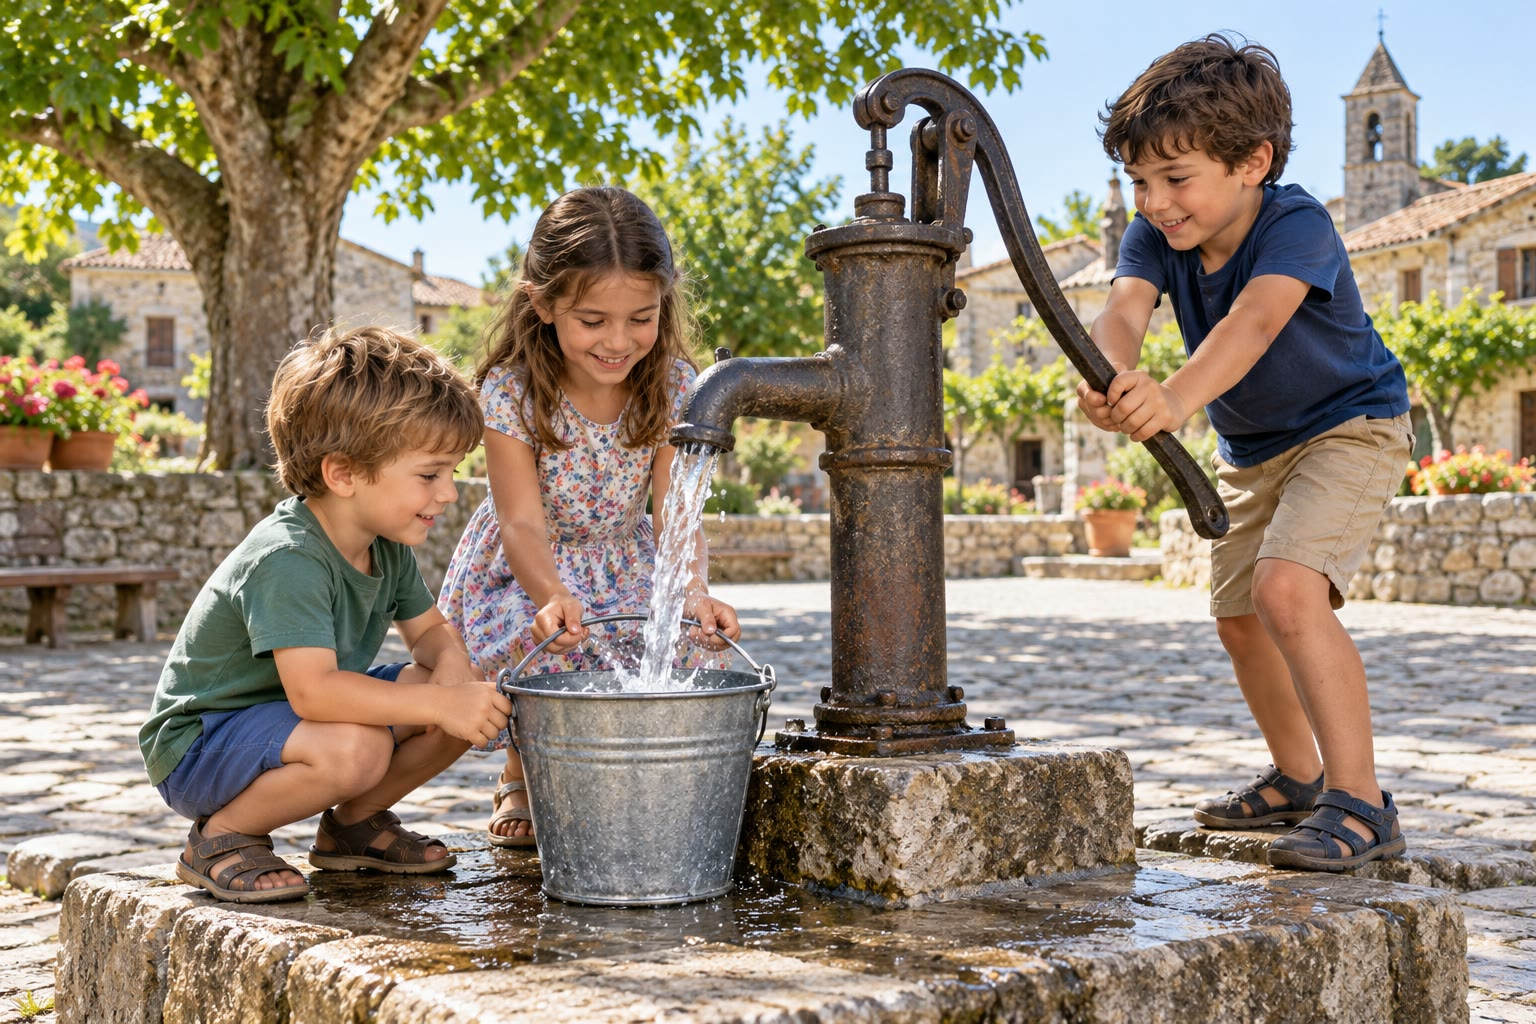
\includegraphics[width=0.6\linewidth]{images/book1/ai/g6-hand-pump.jpg}

{\small बच्चे एक गाँव के \omterm{def:g6:water-underground:spring}{कुएँ} के हैंडपंप पर बाल्टी भरते हैं। (AI
चित्रण।)}
\end{omfigure}

\begin{remark}[कुआँ सूख सकता है]\label{rem:g6:water-underground:pumping}
किसी \omterm{def:g6:water-underground:spring}{कुएँ} से पानी पंप करने पर उसके आसपास \omterm{def:g6:water-underground:water-table}{भौम जलस्तर} नीचे चला जाता है। अगर
पानी उससे ज़्यादा तेज़ी से पंप किया जाए जितनी तेज़ी से \omterm{def:g4:clouds-rain-snow:precipitation}{बारिश} \omterm{def:g3:stones-pebbles-sand:rock}{चट्टान} को फिर से
भरती है, तो \omterm{def:g6:water-underground:water-table}{भौम जलस्तर} नीचे, और नीचे जाता जाता है: \omterm{def:g6:water-underground:spring}{कुआँ} कम से कम पानी देता है
और सूख सकता है। एक ही \omterm{def:g3:stones-pebbles-sand:rock}{चट्टान} से पंप करने वाले दो पड़ोसी एक ही पानी बाँटते हैं:
एक पंप दूसरे का \omterm{def:g6:water-underground:spring}{कुआँ} सुखा सकता है।
% ledger: wss:aquifer
\end{remark}

\section{जलभृत}

\begin{definition}[जलभृत]\label{def:g6:water-underground:aquifer}
\emph{जलभृत}\index{जलभृत} \omterm{def:g6:water-underground:porosity}{सरंध्र} और \omterm{def:g6:water-underground:permeability}{पारगम्य} \omterm{def:g3:stones-pebbles-sand:rock}{चट्टान} की एक परत है, जो \omterm{def:g6:water-underground:groundwater}{भूजल} से
भरी है और इस पानी को \omterm{def:g6:water-underground:spring}{सोतों} और \omterm{def:g6:water-underground:spring}{कुओं} तक बाहर बहने देती है। रिसने वाली \omterm{def:g4:clouds-rain-snow:precipitation}{बारिश}
उसे फिर से भरती है।
% ledger: wss:aquifer
\end{definition}

वार्डन पहाड़ियों की खड़िया एक \omterm{def:g6:water-underground:aquifer}{जलभृत} है: वह \omterm{def:g6:water-underground:porosity}{सरंध्र} है, \omterm{def:g6:water-underground:permeability}{पारगम्य} है, और
\omterm{def:g1:landscapes-around-us:landform}{पहाड़ियों} के फ़ार्म अपना पानी उसी से लेते हैं। उसके नीचे का शेल \omterm{def:g6:water-underground:aquifer}{जलभृत} नहीं
है: पानी उसमें से नहीं बह सकता। और नीचे, शेल के नीचे, एक चूना पत्थर और एक
बलुआ पत्थर हैं, जो भी पानी रख सकते हैं; उस पानी तक पहुँचने के लिए \omterm{def:g6:water-underground:spring}{कुएँ} को
शेल के आर-पार बेधना पड़ता है।

\omterm{def:g6:water-underground:groundwater}{भूजल} जल चक्र का हिस्सा है। \omterm{def:g4:clouds-rain-snow:precipitation}{बारिश} \omterm{def:g6:water-underground:aquifer}{जलभृत} में रिसती है; \omterm{def:g6:water-underground:groundwater}{भूजल} \omterm{def:g6:water-underground:porosity}{रंध्रों} में से
धीरे-धीरे बहता है; वह \omterm{def:g6:water-underground:spring}{सोतों} पर और \omterm{def:g1:landscapes-around-us:water}{नदियों} में बाहर आता है, जो उसे \omterm{def:g2:water-on-earth:ocean}{समुद्र} तक ले
जाती हैं; वहाँ वह वाष्पित होता है, और फिर \omterm{def:g4:clouds-rain-snow:precipitation}{बारिश} बनकर गिरता है। \omterm{def:g6:water-underground:aquifer}{जलभृत} से पानी
लेना ऐसी टंकी से पानी लेने जैसा है जिसे \omterm{def:g4:clouds-rain-snow:precipitation}{बारिश} धीरे-धीरे भरती है: पानी तभी
टिकता है जब हम उससे ज़्यादा न लें जितना \omterm{def:g4:clouds-rain-snow:precipitation}{बारिश} लौटाती है।

\section{भूजल को साफ़ रखना}

ज़मीन में रिसने वाला पानी अपने रास्ते में छनता जाता है: पत्तियाँ, मिट्टी के
कण और छोटे जीव मिट्टी और \omterm{def:g3:stones-pebbles-sand:rock}{चट्टान} में रुक जाते हैं। इसीलिए \omterm{def:g6:water-underground:spring}{सोते} या \omterm{def:g6:water-underground:spring}{कुएँ} का पानी
आमतौर पर बिल्कुल साफ़ दिखता है। पर पानी में \emph{घुले} पदार्थ नहीं रुकते: वे
उसके साथ नीचे \omterm{def:g6:water-underground:water-table}{भौम जलस्तर} तक
चले जाते हैं।
% ledger: wss:gw-quality

लोग ज़मीन पर जो डालते हैं, उससे \omterm{def:g6:water-underground:groundwater}{भूजल} ख़राब हो सकता है: खेतों और बग़ीचों में
छिड़के गए उर्वरक और कीटनाशक, बर्फ़ जमी सड़कों पर डाला गया नमक, किसी टंकी से
रिसता ईंधन, खुले में फेंका गया कचरा, घरों के ठीक से न रखे गए गंदे पानी के टैंकों
से उफनता पानी। \omterm{def:g6:water-underground:aquifer}{जलभृत} में एक बार घुल जाने पर इन पदार्थों को निकालना कठिन होता
है, और हो सकता है कि वह पानी उपचार के बिना पीने लायक न रहे। इसलिए \omterm{def:g6:water-underground:spring}{कुएँ} के पानी
को पीने से पहले जाँचना ज़रूरी है, और उर्वरक, ईंधन और कचरा \omterm{def:g6:water-underground:spring}{कुओं} और \omterm{def:g6:water-underground:spring}{सोतों} से दूर रखना ही सबसे अच्छा है।
% ledger: wss:gw-quality

घुले पदार्थ \omterm{def:g6:water-underground:groundwater}{भूजल} के साथ यात्रा करते हैं। \omterm{def:g6:water-underground:water-table}{भौम जलस्तर} के नीचे पानी धीरे-धीरे
ढलान पर नीचे की ओर सरकता है: वहाँ से जहाँ \omterm{def:g6:water-underground:water-table}{भौम जलस्तर} ऊँचा है, \omterm{def:g1:landscapes-around-us:landform}{पहाड़ियों} के
नीचे, वहाँ तक जहाँ वह नीचा है, \omterm{def:g6:water-underground:spring}{सोतों} और \omterm{def:g1:landscapes-around-us:water}{नदियों} पर। इसलिए ज़मीन पर छलकी और
उसमें रिसी कोई चीज़ वहीं नहीं रहती जहाँ वह गिरी थी। वह नीचे \omterm{def:g6:water-underground:water-table}{भौम जलस्तर} तक जाती
है, फिर \omterm{def:g6:water-underground:groundwater}{भूजल} के साथ ढलान पर नीचे की ओर बहती है, उसकी ओर जो भी ढलान पर उससे
नीचे हो।
% ledger: wss:gw-quality, wss:aquifer

\begin{omfigure}
\begin{tikzpicture}[x=1cm, y=1.15cm, font=\scriptsize]
  % ground (the chalk) and the water-filled zone under the water table
  \fill[black!6] (0,0) -- (0,4.090) -- plot[smooth] coordinates {(0.00,4.090) (1.00,4.013) (2.00,3.887) (3.00,3.692) (4.00,3.407) (5.00,3.033) (6.00,2.600) (7.00,2.167) (8.00,1.793) (9.00,1.508) (10.00,1.313) (11.00,1.187) (12.00,1.110)} -- (12,0) -- cycle;
  \fill[blue!14] (0,0) -- (0,3.190) -- plot[smooth] coordinates {(0.00,3.190) (1.00,3.185) (2.00,3.131) (3.00,3.008) (4.00,2.795) (5.00,2.493) (6.00,2.132) (7.00,1.771) (8.00,1.469) (9.00,1.256) (10.00,1.133) (11.00,1.079) (12.00,1.074)} -- (12,0) -- cycle;
  \draw[black!70, line width=0.7pt] plot[smooth] coordinates {(0.00,4.090) (1.00,4.013) (2.00,3.887) (3.00,3.692) (4.00,3.407) (5.00,3.033) (6.00,2.600) (7.00,2.167) (8.00,1.793) (9.00,1.508) (10.00,1.313) (11.00,1.187) (12.00,1.110)};
  \draw[blue!70!black, dashed, line width=0.7pt] plot[smooth] coordinates {(0.00,3.190) (1.00,3.185) (2.00,3.131) (3.00,3.008) (4.00,2.795) (5.00,2.493) (6.00,2.132) (7.00,1.771) (8.00,1.469) (9.00,1.256) (10.00,1.133) (11.00,1.079) (12.00,1.074)};
  % the spill: down to the water table, then downhill with the groundwater
  \fill[brown!70!black, opacity=0.55] (4.85,3.094) -- (5.15,2.971) -- (5.15,2.442) -- (4.85,2.544) -- cycle;
  \fill[brown!70!black, opacity=0.55] (4.85,2.514) -- (5.10,2.429) -- (5.35,2.341) -- (5.60,2.250) -- (5.85,2.158) -- (6.10,2.065) -- (6.35,1.972) -- (6.60,1.881) -- (6.85,1.792) -- (7.10,1.707) -- (7.35,1.626) -- (7.60,1.549) -- (7.85,1.478) -- (8.10,1.413) -- (8.35,1.354) -- (8.60,1.300) -- (8.85,1.252) -- (9.10,1.210) -- (9.30,1.181) -- (9.10,1.182) -- (8.85,1.190) -- (8.60,1.203) -- (8.35,1.221) -- (8.10,1.246) -- (7.85,1.277) -- (7.60,1.313) -- (7.35,1.355) -- (7.10,1.401) -- (6.85,1.486) -- (6.60,1.598) -- (6.35,1.713) -- (6.10,1.828) -- (5.85,1.945) -- (5.60,2.060) -- (5.35,2.174) -- (5.10,2.286) -- (4.85,2.394) -- cycle;
  % the leaking tank
  \draw[fill=black!35] (4.7,3.10) rectangle (5.3,3.42);
  \node[anchor=south, align=center] at (5.0,3.45) {रिसती\\ईंधन टंकी};
  % groundwater flow
  \begin{scope}[blue!60!black, -{Stealth[length=2mm]}, line width=0.8pt]
    \draw (0.80,2.589) -- (2.40,2.491);
    \draw (3.40,2.334) -- (5.00,1.893);
    \draw (5.90,1.569) -- (7.50,1.009);
    \draw (8.80,0.691) -- (10.60,0.494);
  \end{scope}
  \node[blue!60!black, anchor=north] at (6.7,1.0) {भूजल ढलान पर नीचे बहता है};
  % the two wells
  \draw[line width=1.6pt, black!75] (2.0,3.887) -- (2.0,2.70);
  \draw[line width=1.6pt, black!75] (8.5,1.639) -- (8.5,0.95);
  \node[anchor=south, align=center] at (2.0,3.95) {कुआँ A\\(ऊपर की ओर): साफ़};
  \draw[black!50] (8.5,1.66) -- (8.5,2.30);
  \node[anchor=south, align=center] at (8.5,2.30) {कुआँ B\\(नीचे की ओर): ख़राब};
  % the stream
  \fill[blue!60] (11.55,1.13) -- (11.95,1.11) -- (11.75,1.02) -- cycle;
  \node[anchor=south] at (11.6,1.20) {नाला};
  \node[blue!70!black, anchor=south west] at (0.1,3.21) {भौम जलस्तर};
  \node[anchor=west, black!70] at (0.15,0.25) {खड़िया};
\end{tikzpicture}

{\small एक \omterm{def:g1:landscapes-around-us:landform}{पहाड़ी} ढलान पर छलका ईंधन (एक रेखाचित्र)। घुला हुआ ईंधन नीचे \omterm{def:g6:water-underground:water-table}{भौम
जलस्तर} तक जाता है, फिर \omterm{def:g6:water-underground:groundwater}{भूजल} के साथ ढलान पर नीचे की ओर बहता है (नीले तीर): वह
ढलान पर उससे नीचे वाले \omterm{def:g6:water-underground:spring}{कुआँ} B तक, और अंत में नाले तक पहुँचता है। टंकी से ऊपर
की ओर वाला \omterm{def:g6:water-underground:spring}{कुआँ} A साफ़ रहता है।}
\end{omfigure}

\begin{method}[क्या कोई कुआँ ख़तरे में है?]\label{met:g6:water-underground:risk}
\begin{enumerate}
  \item पता करो कि \omterm{def:g6:water-underground:water-table}{भौम जलस्तर} कहाँ ऊँचा है और कहाँ नीचा: वह \omterm{def:g1:landscapes-around-us:landform}{पहाड़ियों} के
        नीचे ऊँचा और \omterm{def:g6:water-underground:spring}{सोतों} और \omterm{def:g1:landscapes-around-us:water}{नदियों} के पास नीचा होता है।
  \item \omterm{def:g6:water-underground:groundwater}{भूजल} ऊँचे से नीचे की ओर बहता है: उसकी दिशा एक तीर से
        बनाओ।
  \item जो \omterm{def:g6:water-underground:spring}{कुआँ} या \omterm{def:g6:water-underground:spring}{सोता} प्रदूषण के किसी स्रोत से ढलान पर नीचे, उस तीर के
        रास्ते पर है, वह ख़तरे में है; उससे ऊपर की ओर वाला \omterm{def:g6:water-underground:spring}{कुआँ} नहीं।
\end{enumerate}
\end{method}

\begin{example}[फ़ार्म के लिए एक नई ईंधन टंकी]\label{ex:g6:water-underground:tank}
खड़िया की एक \omterm{def:g1:landscapes-around-us:landform}{पहाड़ी} ढलान पर एक किसान अपने ही \omterm{def:g6:water-underground:spring}{कुएँ} का पानी पीती है, जो ढलान
के बीच में है, और दो खेतों में से किसी एक में एक नई ईंधन टंकी रखना चाहती है:
एक खेत \omterm{def:g6:water-underground:spring}{कुएँ} से ऊपर की ओर है, एक उससे नीचे की ओर, नाले के पास। \omterm{def:g6:water-underground:groundwater}{भूजल} ढलान पर
नीचे की ओर बहता है। ऊपर वाले खेत से रिसाव नीचे \omterm{def:g6:water-underground:spring}{कुएँ} की ओर बहेगा; नीचे वाले
खेत से रिसाव \omterm{def:g6:water-underground:spring}{कुएँ} से दूर, नाले की ओर बहेगा। \omterm{def:g6:water-underground:spring}{कुएँ} के लिए नीचे वाला खेत बेहतर
विकल्प है --- और ऐसी ट्रे पर रखी टंकी, जो कोई भी रिसाव रोक ले, और भी बेहतर
है, क्योंकि नाला भी मायने रखता
है।
\end{example}

\begin{inthefield}[सोते पहचानना]
किसी बड़े के साथ सैर पर किसी ढलान की तलहटी के साथ-साथ देखो। \omterm{def:g6:water-underground:spring}{सोता} अक्सर गीली
ज़मीन के एक टुकड़े के रूप में, किसी सूखे खेत में ज़्यादा हरी घास या सरकंडों की एक
कतार के रूप में, कहीं से भी शुरू होते एक छोटे नाले के रूप में, या पानी पकड़ने
के लिए बने पत्थर के कुंड या नाँद के रूप में दिखाई देता है। पैदल रास्तों के
विस्तृत \omterm{def:g2:drawing-to-map:map}{मानचित्र} पर \omterm{def:g6:water-underground:spring}{सोते} एक छोटे प्रतीक से दिखाए जाते हैं। रास्ते से ही देखो:
किसी ऐसे \omterm{def:g6:water-underground:spring}{सोते} का पानी कभी मत पियो जिसकी जाँच न हुई हो।
\end{inthefield}

\section{अभ्यास}

\begin{exercise}[$\star$]\label{exo:g6:water-underground:1}
इन पदार्थों को ``\omterm{def:g6:water-underground:permeability}{पारगम्य}'' और ``\omterm{def:g6:water-underground:permeability}{अपारगम्य}'' में छाँटो: \omterm{def:g3:stones-pebbles-sand:sand}{रेत}, चिकनी मिट्टी,
\omterm{def:g3:stones-pebbles-sand:pebble}{बजरी}, बिना दरारों वाला ग्रेनाइट, शेल, खड़िया।
\end{exercise}

\begin{exercise}[$\star$]\label{exo:g6:water-underground:2}
हर शब्द को उसके अर्थ से मिलाओ: \omterm{def:g6:water-underground:spring}{सोता}; \omterm{def:g6:water-underground:spring}{कुआँ}; \omterm{def:g6:water-underground:water-table}{भौम जलस्तर}; \omterm{def:g6:water-underground:aquifer}{जलभृत}।
(क) उस क्षेत्र की ऊपरी सीमा जहाँ सारे \omterm{def:g6:water-underground:porosity}{रंध्र} पानी से भरे हैं। (ख) एक \omterm{def:g6:water-underground:porosity}{सरंध्र}
और \omterm{def:g6:water-underground:permeability}{पारगम्य} परत जो \omterm{def:g6:water-underground:groundwater}{भूजल} रखती है। (ग) एक जगह जहाँ \omterm{def:g6:water-underground:groundwater}{भूजल} अपने-आप बाहर आता
है। (घ) एक छेद जो \omterm{def:g6:water-underground:water-table}{भौम जलस्तर} के नीचे तक
जाता है।
\end{exercise}

\begin{exercise}[$\star$]\label{exo:g6:water-underground:3}
(क) उन तीन रास्तों के नाम बताओ जो ज़मीन पर गिरने वाला \omterm{def:g4:clouds-rain-snow:precipitation}{बारिश} का पानी ले सकता
है। (ख) \omterm{def:g5:natural-hazards:storm}{तूफ़ान} के बाद ज़्यादा पानी कहाँ बहता है: कार पार्किंग पर या घास के
मैदान पर? क्यों?
\end{exercise}

\begin{exercise}[$\star$]\label{exo:g6:water-underground:4}
सही या ग़लत? ग़लत वाक्यों को सुधारो। (क) \omterm{def:g6:water-underground:porosity}{सरंध्र} \omterm{def:g3:stones-pebbles-sand:rock}{चट्टान} हमेशा \omterm{def:g6:water-underground:permeability}{पारगम्य} होती
है। (ख) \omterm{def:g6:water-underground:water-table}{भौम जलस्तर} के नीचे \omterm{def:g6:water-underground:porosity}{रंध्र} पानी से भरे होते हैं। (ग) \omterm{def:g6:water-underground:water-table}{भौम जलस्तर} किसी
\omterm{def:g1:landscapes-around-us:water}{झील} की सतह की तरह समतल होता है। (घ) सारी \omterm{def:g1:landscapes-around-us:water}{झीलों} की तुलना में ज़मीन के नीचे
ज़्यादा \omterm{def:g2:water-on-earth:salt-fresh}{मीठा पानी} है।
\end{exercise}

\begin{exercise}[$\star\star$]\label{exo:g6:water-underground:5}
एक बाल्टी में 10~लीटर सूखी \omterm{def:g3:stones-pebbles-sand:sand}{रेत} है। \omterm{def:g3:stones-pebbles-sand:sand}{रेत} की \omterm{def:g6:water-underground:porosity}{सरंध्रता} 25~\% है। बाल्टी के
उफनने से पहले तुम उसमें कितना पानी डाल सकते हो? तली के एक छेद से कितना पानी
बाहर निकलेगा (22~\%)?
\end{exercise}

\begin{exercise}[$\star\star$]\label{exo:g6:water-underground:6}
चूना पत्थर का एक खंड 2~मीटर गुणा 1~मीटर गुणा 1~मीटर का है। (क) घन मीटर में और
लीटर में उसका आयतन कितना है? (ख) उसकी \omterm{def:g6:water-underground:porosity}{सरंध्रता} 20~\% है: भरा होने पर वह कितने
लीटर पानी रखता है? (ग) इस पानी में से खंड के आयतन का 18~\% बाहर निकल जाता है।
कितने लीटर बाहर निकलते हैं, और कितने अटके रहते हैं?
\end{exercise}

\begin{exercise}[$\star\star$]\label{exo:g6:water-underground:7}
वार्डन पहाड़ियों से होकर जाने वाली काट का उपयोग करो। (क) \omterm{def:g6:water-underground:spring}{सोता} किस ऊँचाई पर
है? और \omterm{def:g1:landscapes-around-us:water}{नदी}? (ख) \omterm{def:g6:water-underground:spring}{सोता} \omterm{def:g1:landscapes-around-us:water}{नदी} से ऊपर है या नीचे? \omterm{def:g6:water-underground:spring}{सोते} का पानी कहाँ जाता है?
(ग) खड़िया की \omterm{def:g1:landscapes-around-us:landform}{पहाड़ी} ढलान के बीच में कोई \omterm{def:g6:water-underground:spring}{सोता} क्यों नहीं है?
\end{exercise}

\begin{exercise}[$\star\star$]\label{exo:g6:water-underground:8}
\omterm{def:g6:water-underground:spring}{कुएँ}~A के पास ज़मीन 401~मीटर पर है; \omterm{def:g6:water-underground:water-table}{भौम जलस्तर} बरसात के मौसम के बाद 336~मीटर पर
और सूखे मौसम के बाद 314~मीटर पर होता है। (क) हर मौसम में पानी ज़मीन से कितना
नीचे है? (ख) दोनों मौसमों के बीच \omterm{def:g6:water-underground:water-table}{भौम जलस्तर} कितने मीटर नीचे जाता
है?
\end{exercise}

\begin{exercise}[$\star\star$]\label{exo:g6:water-underground:9}
एक किसान \omterm{def:g1:landscapes-around-us:landform}{पहाड़ी} की चोटी पर, काट के दाएँ सिरे पर, एक नया \omterm{def:g6:water-underground:spring}{कुआँ} चाहता है। यह \omterm{def:g6:water-underground:spring}{कुआँ}
\omterm{def:g6:water-underground:spring}{कुएँ}~A से ज़्यादा गहरा होना चाहिए या कम? \omterm{def:g6:water-underground:water-table}{भौम जलस्तर} की मदद से
समझाओ।
\end{exercise}

\begin{exercise}[$\star\star$]\label{exo:g6:water-underground:10}
एक घन मीटर चिकनी मिट्टी 500~लीटर पानी रखती है पर केवल 20~लीटर देती है।
समझाओ कि चिकनी मिट्टी में खोदा गया \omterm{def:g6:water-underground:spring}{कुआँ} लगभग कोई पानी क्यों नहीं देता, जबकि
चिकनी मिट्टी पानी से भरी होती है।
\end{exercise}

\begin{exercise}[$\star\star\star$]\label{exo:g6:water-underground:11}
पृथ्वी के सारे \omterm{def:g2:water-on-earth:salt-fresh}{मीठे पानी} में से 30.1~\% \omterm{def:g6:water-underground:groundwater}{भूजल} है और 0.26~\% \omterm{def:g1:landscapes-around-us:water}{झीलों} में है।
(क) \omterm{def:g1:landscapes-around-us:water}{झीलों} की तुलना में ज़मीन के नीचे कितने गुना ज़्यादा \omterm{def:g2:water-on-earth:salt-fresh}{मीठा पानी} है? (ख) सारे
\omterm{def:g2:water-on-earth:salt-fresh}{मीठे पानी} में से लगभग 69~\% बर्फ़ और \omterm{def:g4:clouds-rain-snow:precipitation}{हिम} है। बाकी सब (\omterm{def:g6:water-underground:groundwater}{भूजल}, \omterm{def:g1:landscapes-around-us:water}{झीलें}, \omterm{def:g1:landscapes-around-us:water}{नदियाँ},
हवा, मिट्टी\ldots) के लिए कितना हिस्सा बचता है? (ग) पीने के पानी के लिए \omterm{def:g6:water-underground:groundwater}{भूजल}
इतना महत्वपूर्ण क्यों है?
\end{exercise}

\begin{exercise}[$\star\star\star$]\label{exo:g6:water-underground:12}
दो फ़ार्म एक ही खड़िया पर अगल-बगल हैं। एक गर्मी में पहला फ़ार्म एक शक्तिशाली
पंप लगाता है और एक बड़ा तालाब भरता है; कुछ हफ़्ते बाद दूसरे फ़ार्म का \omterm{def:g6:water-underground:spring}{कुआँ}
सूख जाता है, हालाँकि किसी ने उसे छुआ तक नहीं। समझाओ कि क्या हुआ, और दोनों
किसान क्या कर सकते हैं।
\end{exercise}

\section{समस्या: वार्डन पहाड़ियों में एक फ़ार्म का कुआँ}

\begin{problem}[{सप्ताहांत समस्या --- वार्डन पहाड़ियों के एक फ़ार्म के नीचे
की चट्टानें, उसकी खड़िया में जमा पानी, और बिना बारिश के वह कितने दिन
चलेगा}]
\label{pb:g6:water-underground:1}
% ledger: heath:porosity, wss:aquifer
वार्डन पहाड़ियों का एक फ़ार्म खड़िया पर, काट के \omterm{def:g6:water-underground:spring}{कुएँ}~A के पास है। किसान जानना
चाहता है कि एक लंबे सूखे में, अगर खड़िया को फिर से भरने के लिए बिल्कुल भी
\omterm{def:g4:clouds-rain-snow:precipitation}{बारिश} न हो, तो \omterm{def:g6:water-underground:spring}{कुआँ} फ़ार्म का काम कितने समय तक चला सकता है।

\medskip
\noindent\textbf{भाग I --- फ़ार्म के नीचे की चट्टानें।}
\begin{enumerate}
  \item उस \omterm{def:g3:stones-pebbles-sand:rock}{चट्टान} का नाम बताओ जिस पर फ़ार्म है, और उसके नीचे वाली \omterm{def:g3:stones-pebbles-sand:rock}{चट्टान} का।
        कौन-सी \omterm{def:g6:water-underground:permeability}{पारगम्य} है?
  \item समझाओ कि फ़ार्म के नीचे ढलान की तलहटी पर \omterm{def:g6:water-underground:spring}{सोता} क्यों बहता है।
  \item काट का उपयोग करो: फ़ार्म पर ज़मीन 401~मीटर पर है और बरसात के मौसम के
        बाद \omterm{def:g6:water-underground:water-table}{भौम जलस्तर} 336~मीटर पर है। पानी कितना नीचे है?
  \item सूखे मौसम के बाद \omterm{def:g6:water-underground:water-table}{भौम जलस्तर} 314~मीटर पर है। \omterm{def:g6:water-underground:spring}{कुआँ}~A 100~मीटर
        गहरा है। क्या वह अब भी पानी तक पहुँचता है? कितने मीटर से?
\end{enumerate}

\medskip
\noindent\textbf{भाग II --- खड़िया में पानी।}
किसान \omterm{def:g6:water-underground:spring}{कुएँ} के आसपास खड़िया के एक खंड से पानी निकाल सकता है, जो \omterm{def:g6:water-underground:water-table}{भौम जलस्तर} के
नीचे है और 100~मीटर लंबा, 50~मीटर चौड़ा और 2~मीटर मोटा है। खड़िया एक चूना पत्थर
है: 20~\% \omterm{def:g6:water-underground:porosity}{सरंध्रता} और 18~\% बाहर निकलने वाले पानी का हिस्सा मानो।
\begin{enumerate}[resume]
  \item खंड का आयतन घन मीटर में कितना है?
  \item उसके \omterm{def:g6:water-underground:porosity}{रंध्रों} को कितने घन मीटर पानी भरता है?
  \item उसमें से कितने घन मीटर पानी बाहर निकलकर \omterm{def:g6:water-underground:spring}{कुएँ} में आता है? कितना
        खड़िया में अटका रहता है?
  \item बाहर निकलने वाले पानी को लीटर में लिखो।
\end{enumerate}

\medskip
\noindent\textbf{भाग III --- पानी कितने समय चलता है।}
\begin{enumerate}[resume]
  \item फ़ार्म (घर, जानवर और सब्ज़ियों का बग़ीचा) रोज़ 18~घन मीटर पानी
        इस्तेमाल करता है। यह कितने लीटर है?
  \item फ़ार्म एक हफ़्ते में कितना पानी इस्तेमाल करता है?
  \item सामान्य वर्ष में खड़िया में पानी का भंडार ख़त्म क्यों नहीं होता?
  \item बिल्कुल भी \omterm{def:g4:clouds-rain-snow:precipitation}{बारिश} न हो, तो खंड से बाहर निकलने वाला पानी फ़ार्म को कितने
        दिन तक पानी दे पाएगा?
\end{enumerate}
\end{problem}
